\chapter{Results}
\label{ch:result}

In this chapter we will discuss the results retrieved after applying our LDA implementation. Section \ref{results:evaluation measures} defines the 4 different evaluation measures. In section \ref{results:modelresults} our results will be shown. Furthermore section \ref{results:parameter tuning} present the tuning results.

\section{Model results}\label{results:modelresults}


\begin{figure}[h]
    \centering
    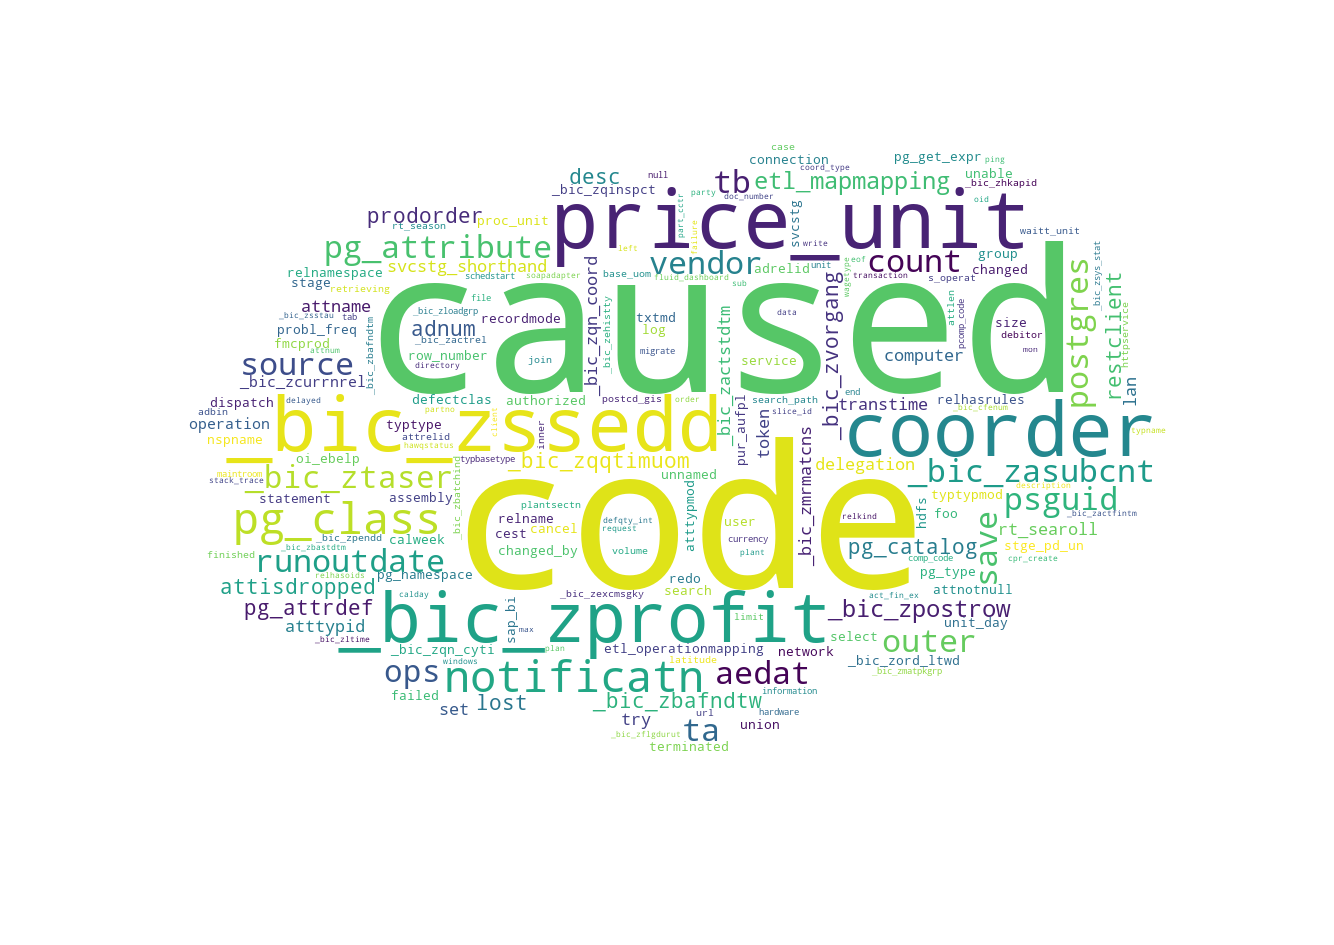
\includegraphics[width=15cm, height=8cm]{figures/wc.png}
    \caption{A wordcloud containing terms found in clusters}
    \label{fig:worldcloud}
\end{figure}

\begin{comment}

The model used is ofcourse LDA.

\end{comment}

\section{Evaluation Measures}\label{results:evaluation measures}
To evaluate our implementation we use different metrics. Evaluating an unsupervised learning model depends on the application and the goal the model is made with. In our case the metrics are here to evaluate the models capability to generalise, using perplexity. The clusters are evaluated based on their inner similarity between documents and \" distance \" compared to other cluster centroids, using Silhouette co\"efficient. The distance metric used for silhouette co\"efficient is based on the KL-divergence metric. The last measurement we use is coherence in topics and the measurement of distance between topic document clusters using the visual tool LDAvis.

\subsection{Perplexity}\label{research:perplexity}
In the original paper Blei introduces a general model evaluation metric \cite{Blei2003} to compare topic models. Perplexity can be used to compare the generalisation of a model on new unlabelled data.

\[
   \mathlarger{perplexity(\textbf{D}_{test}) = \exp{\Bigg \{ -\frac{\sum{}_{d=1}^{M}logp(\textbf{w}_d)}{\sum{}_{d=1}^{M}N_d} \Bigg \}}}
\]

Perplexity shows the perplexity on the test set of held out documents $\textbf{D}$. The nominator shows the sum in  corpus $M$ with document $d$, where the likelihood of each word in d is computed. The denominator consists of the count of words $N$ in document $d$.
The lower the perplexity score the better a model generalises. 


\subsection{Silhouette coefficient} \label{research:silhouette}
The silhouette is used to measure between the cohesion and the separation of intra-clusters. In our model this measures the mean intra-cluster distance for each document and compares distance to the nearest-cluster distance.

\[
   \mathlarger{s(i) = \frac{b(i) - a(i)}{\max{\{ a(i), b(i)}\} } }
\]

Where $s_i$ is the silhouette of sample $i$ in the cluster. $a_i$ is the average distance for $i$ from all the objects in the cluster and $b_i$ the distance of $i$ from a cluster $b$ not containing $i$. 

\[
\mathlarger{-1 \leq s \le 1}
\]

The value of $s$ will be contained between $-1$ and $1$. If $s(i) = 1$ then we can say that the distance $i$  is a lot less in its own cluster then the nearest other cluster. If we take $s(i) = -1$ then the similarity of $i$ is higher in the other nearest cluster then its current cluster \cite{Rousseeuw1987Silhouettes:Analysis}.


\subsection{Jensen-Shannon divergence and KL-divergence} \label{research:jsdivergence}
The Kullback Leiber divergence was introduced to measure the density between to distributions \cite{Hershey2007ApproximatingModels}. Based upon this important and popular measure the Jensen-Shannon divergence (JS) was introduced \cite{Fuglede2004Jensen-ShannonEmbedding}. Which is better used to measure similarity between two text documents based on their probability distributions.

\[
\mathlarger{JDS(P||Q) = \frac{1}{2}D(P||M) + \frac{1}{2}D(Q||M)}
\]

Where $P$ and $Q$ denote a probability distribution and $M$ the set of probability distributions. The useful if especially to find the distinctiveness and cohesion between topics

\subsection{Human perception}\label{results:humanperception}
Although LDA can be used to find latent patterns, explore, tag recommend in a document corpus the final result of topics do not necessarily match up with the human expectation of a topic. Especially in a unsupervised learning model with only mathematical measures\cite{Towne2016MeasuringPerception}. The reason of this paragraph is to make readers aware that the suitability of a model in a unsupervised learning and NLP environment still need support of a human factor. Research from Chang  et al. \cite{Chang2009ReadingModels} and Blei et al. \cite{Chaney2012VisualizingModels.} provide more in depth research in this topic.  

With that in mind, the highly dimensional LDA is actually suitable in contrast to most machine learning techniques to be evaluated using visual tools. One such tool is LDAvis, a tool that got developed in R and D3 \cite{Sievert2014}. LDAvis is a web-based interactive visual of the topics on a fitted LDA model. The multidimensional LDA is scaled to two dimensions, making it possible to visually see the distance between topics and quickly determine their distinctiveness. Simultaneously the visual tool shows the relevance of each term in their selected topic, based on their exclusiveness and occurs within that topic compared to different topics.

\subsection{parameter tuning}\label{results:parameter tuning}
During the experimental phase. The research coneducted sucked, but Althought it sucked we got somewhere. 

\section{Graphs of results}

\begin{comment}
Visualizing the messages is really fun!
\end{comment}

\section{Contribution}\label{results:contribution}



\begin{comment}
I dont think I contributed a lot to the research in this area, but I learned a lot right??
\end{comment}
